% !TEX root = MAIN.tex

\clearpage
\section{Code-driven Mutation Testing}
\label{sec:back:testGeneration}

This section describes the approaches that can be adopted to automatically generate test cases that kill mutants.
To kill a mutant we need test cases that (1) reach the mutation point (i.e., execute the mutated code), (2) cause 
corruptions
in the program state right after the mutated code,
and (3) manifest these corruptions into the program output 
(e.g., by producing an erroneous value in a state variable verified by a test assertion) 
thus leading to a failure~\cite{papadakis2019mutation}. These conditions are also known as the \INDEX{killing conditions} of a mutant.

In the literature, there exist two groups of approaches for 
generating test cases that kill mutants:
approaches based on constraint-programming, and approaches based on evolutionary computation. Below we introduces these two stream of approaches after introducing two well-known solutions for test generation driven by structural coverage, which are the basis for mutation testing solutions based on constraint programming.

\subsection{Test Generation driven by program structure}
\label{sec:back:generation:structure}
Two alternative state-of-the-art solutions to generate test inputs that maximize structural coverage are CBMC, a bounded model checker, and KLEE~\cite{cadar2008klee}, a symbolic execution engine. They are detailed below.

%\subsubsection{CBMC}
%\label{subsec:cbmc}

\INDEX{CBMC} is an approach that implements \INDEX{Bounded Model Checking}~\cite{BiereCCZ:TACAS99,SeryFS:ATVA12} (BMC), an approach for purely static software verification.
The idea in BMC is to represent the software together with the
properties to be verified as an instance of the propositional
satisfiability problem (SAT).  Such a representation captures the
software behavior exactly, assuming that all the loop bodies in the
software are repeated at most a fixed number of times.
This approach has several advantages: the logical formulation is usually
very compact compared to traditional model checking, where verification
is reduced to a reachability problem in a graph representing the program
state space;
%
there are several high-performance SAT
solvers~\cite{MarquesSilva:IEEETRAN99,EenS:SAT2003} that can be used for
solving the instances;
%
and the satisfying assignments of an instance can be directly translated
to meaningful counterexamples for correctness in the form of
fault-inducing executions.
%
Furthermore, it is widely recognized that BMC based approaches are particularly good
at quickly finding short counterexamples when they exist.

%A {\em bounded model checker} takes as input a program $\prog$, a bound $k$
%for loop unrolling, and a set $S$ of properties to be verified against
%$\prog$, and returns for each property ${l}$ in $S$, expressed as a propositional statement over variables of $\prog$ at a location $l$, either \vspace{-0.2cm}
%\begin{itemize}
%    \item \emph{verified}, if the executions of $\prog$  satisfy $\prop{l}$;\vspace{-0.25cm}
%    \item \emph{unreachable}, if no execution of $\prog$ reaches $l$;\vspace{-0.25cm}
%    \item \emph{false}, if there is an execution of $\prog$
%    where the property $l$ is broken; and\vspace{-0.25cm}
%    \item \emph{unknown}, if the checker is unable, due to
%    memory or time limits, to determine whether ${l}$ holds,\vspace{-0.2cm}
%\end{itemize}
%under the assumption that no loop body in the program is repeated more
%than $k$ times.
%
%The approach is naturally a compromise between practicality and
%completeness.
%As the SAT problem is \INDEX{NP-complete}, determining whether $\prop{l}$ holds
%requires in the worst case exponential time with respect to the size of
%the SAT instance for all known algorithms.
%%
%Furthermore, the instances can in some cases grow very large since many
%operations, such as multiplication, have quadratic encodings in SAT and,
%for example, the instance grows exponentially in number of nested loops.
%%
%
%Due to numerous optimizations BMC can nevertheless solve many practical
%problems in reasonable time and memory limits.
%%
%For example, the size of the resulting SAT instance can be dramatically
%reduced by slicing off parts of the program that do not affect the
%validity of the property being checked, and
%%
%extremely efficient SAT solver implementations which learn the instance
%structure and use adaptive heuristics~\cite{MahajanFM:SAT04} rarely
%suffer from the exponential worst-case behavior in problems emerging
%from applications.
%%
%The fact that bounded model checkers only prove correctness of
%properties for executions not exceeding the bound $k$ is also beneficial
%in many ways for detecting regressions.  In addition to obvious
%performance benefits our experiments show that in most cases even a single
%loop iteration is sufficient to indicate a regression between two
%versions, and a small bound guarantees in a natural way that the
%reported counterexamples are short.

%\subsubsection{KLEE}

\INDEX{KLEE}~\cite{cadar2008klee} is an open source tool that implements {\INDEX{Concolic Execution}}, a technique that performs \INDEX{symbolic execution} along a concrete execution path. KLEE was designed to automatically generate test cases that achieve high code coverage. The tool is implemented as a modified LLVM virtual machine that targets LLVM bytecode programs.
KLEE also provides a symbolic POSIX library that enable analysis of programs that uses the system's environment. For example, KLEE can be executed with the flag \texttt{-sym-stdin N} which will make stdin symbolic with size \texttt{N}.  

In FAQAS, we rely on KLEE to automatically produce the inputs that make the mutated version of the program generate a different output than the original version.



\subsection{Test Generation based on Constraint Programming}
\label{sec:testGen:CP}

Techniques based on constraint programming use some form of automated reasoning (e.g., Propositional Satisfiability or Constraint Solving~\cite{SATandCPsurvey:2006}) to derive data that satisfy all the conditions necessary to kill a mutant~\cite{offutt1997automatically}.Existing approaches, differ for the strategy adopted to automatically generate these constraints from the program under test.

Offutt et al.~\cite{offutt1997automatically}, for example, automatically derive such constraints from the program by extracting the predicate expressions on the program's control flow graph.
Then, such constraints are encoded to form a constraint system. In their approach, they propose three strategies for identifying infeasible constraint systems, the contradictions to such systems are the new test cases for the program under analysis.

% !TEX root =  ../MutationTestingSurvey.tex

\begin{lstlisting}[style=CStyle, caption=midval function returns the mid value between three integers., label=midval, mathescape=true]
int midval (int x, int y, int z) {
	int midval;

	midval = z;
	if (y < z) {
		if (x < y) {
			midval = y;
		}
		else if (x < z) 
 $\Delta$ else if (x <= z) {
			midval = x;	
		}
	}
	else 
		if (x > y) {
			midval = y;
		} else if (x > z) {
			midval = x;
		}
	return midval;
}
\end{lstlisting}

In the following, we introduce an example of the application of Offutt's~\cite{offutt1997automatically} approach by using the \texttt{midval} function presented in Listing~\ref{midval}. This function has a mutation on line 9, which has been mutated into line 10. According to their approach, the three killing conditions would be the following:

\begin{itemize}
	\item Reachability $C_R: (y < z) \wedge (x \geq y)$
	\item Necessity $C_N: (x < z) \neq (x \leq z)$
	\item Sufficiency $C_S:$ Output(P) $\neq$ Output(M)
\end{itemize}

$C_R$ defines the condition required to reach the mutated statement, in this case the conjunction between the predicate of the first if condition and the negation of the second if condition. $C_N$ defines the condition required to assure a different program state between the original and mutated version of the program right after the mutation point. Finally, $C_S$ defines the condition necessary to demonstrate that both the original and the mutated program returns different values.

Holling et al.~\cite{holling2016nequivack} proposed to use a \INDEX{symbolic execution} approach to identify new test cases. Their idea is to first execute symbolically both the original and the mutated function, then to check if their return values are equivalent or not. 
Symbolic execution determines what inputs cause each part of a function to be covered during execution. To symbolically execute a function, it is necessary to replace the original inputs (i.e., concrete values) with symbolic ones. The \INDEX{symbolic values} represent a set of possible concrete values that lead to a certain program path (i.e., path condition). 


Holling's approach~\cite{holling2016nequivack} to automatically identify equivalent mutants relies on the observation that 
two mutants are equivalent when there are no concrete values making the mutated function produce an output that is different from the one of the original function.
If a value that makes the two functions generate distinct results can be found, the mutant is non-equivalent.
To automate the generation of inputs, Holling et al. rely on KLEE~\cite{cadar2008klee}.

We introduce an example of Holling's approach in Listing~\ref{function}. The top part of Listing~\ref{function} shows the function \texttt{isPositive}, which checks if an integer number is positive or not. The bottom part of Listing~\ref{function} presents the mutated version of \texttt{isPositive}, where the relational operator $\geq$ has been replaced by the operator $>$.
To automate the generation of inputs using KLEE, all the parameters need to be treated as symbolic values.
%F: "the \texttt{isPositive} parameter \texttt{num}" it's impossible to understand what is the parameter and who owns the parameter
%In Holling's approach, first, the \texttt{isPositive} parameter \texttt{num} needs to be treated as symbolic value, which is done by the function \texttt{make\_symbolic} (see Listing~\ref{example}) which converts concrete variables to symbolic by considering its memory address and size. 
This is achieved by function \texttt{make\_symbolic} (see Listing~\ref{example}) which converts concrete variables to symbolic ones by considering their memory address and size. 
%F: please fix
In Listing~\ref{example}, the parameter \texttt{numSymbolic} is made symbolic in Line 3. Then, the original and mutated functions are called using the symbolic arguments in Lines 5 and 6.
%Finally, the \texttt{assert} function of line 8 verifies if the integer return values of both functions are equal or not.
Finally, we need to introduce an assertion that makes the symbolic execution engine \EMPH{look for inputs that make the output of the two functions different}. 
In Listing~\ref{example}, this is achieved with an assertion that verifies that the return values of the two functions the same (see Line 8). 
Despite being counter-intuitive, this approach is effective because symbolic execution engines aim to identify inputs that falsify the assertions in the program. 
When the equality is falsified, then the two functions can produce a different output for a same input.
The input that falsifies the equality can thus be used to improve the test suite enabling it to kill the mutant.
In the example of Listing~\ref{example}, KLEE will indicate that the return values of the original and mutated function differ when \texttt{num} is equal to zero.
A new test case exercising function \texttt{isPositive} with \texttt{num=0} should thus be added to the test suite in order to kill the mutant.

\begin{lstlisting}[style=CStyle, caption=isPositive and MUT\_isPositive functions, label=function]
int isPositive(int num){
	if (num >= 0){
		return 1;
	} else {
		return 0;
	}
}

int MUT_isPositive(int num){
	if (num > 0){
		return 1;
	} else {
		return 0;
	}
}

\end{lstlisting}

\begin{lstlisting}[style=CStyle, caption=Holling's approach for test case generation., label=example]
void test () { 
	int numSymbolic; 
	make_symbolic(&numSymbolic, sizeof(numSymbolic), "numSymbolic"); 
 	
 	int original_ret = isPositive(numSymbolic); 
	int transformed_ret = MUT_isPositive(numSymbolic); 
 
	assert(original_ret == transformed_ret); 
}
\end{lstlisting}

Similarly to Holling's approach, Riener et al.~\cite{riener2011test} proposed to use \INDEX{bounded model checking} techniques to search for these counter examples.
In their bounded model checking approach, the original program and the mutant are unrolled with respect to a certain maximum bound. In program unrolling, loops are re-written as a repeated sequence of similar independent statements. Then, both unrolled programs are encoded into a logic formula over the same input variables. To ensure that the mutation affects the output of the mutant, a propagation condition is encoded and added to the previous logic formula, the condition asserts that there exist at least one pair of different outputs under the assumption of equal inputs. In the last step, the formula is processed by a SMT-solver, if the solver finds a satisfying assignment, the inputs of the formula are translated into a new test case for the current program under analysis.

%Compared to symbolic execution, one advantage of bounded model checking is that it does not require to execute the whole program but may focus on the mutated functions only.

%To reduce the time required by the symbolic execution process, which needs to be performed against all the mutants of the software, Papadakis et al.~\cite{papadakis2011automatically, papadakis2010towards} propose to combine symbolic execution techniques and \INDEX{mutant schemata} to automatically generate test cases targeting the killing conditions induced by the different mutants embedded into the same executable. The approach targets \INDEX{weak mutation} testing and may not generalize to strong mutation testing. Indeed, ensuring the sufficiency property (i.e., verify that changes are propagated to outputs) for multiple mutants might lead to scalability issues not addressed by the proposed approach.





\INDEX{SEMu}~\cite{chekam2021killing} is a recent mutantion testing  framework based on dynamic symbolic execution that has been built on top of the KLEE Symbolic Virtual Machine~\cite{cadar2008klee}.
SEMu uses a form of \INDEX{differential symbolic execution}~\cite{person2008differential} to generate test inputs that kill mutants. The approach consists of modeling the mutant killing problem as a symbolic execution search in a scalable and cost-effective way. 
The SEMu framework is the building block of 
%act as a baseline for 
the test generation tool developed in FAQAS (i.e., \INDEX{SEMuS}). Different from the approaches presented above, SEMu can generate test inputs that kill mutants without the need of human intervention (e.g., to ad assertions); however, it targets only bash programs, it cannot generate unit test cases, for example.

%To kill a mutant, we need test cases that capture the three killing conditions of a mutant~\cite{offutt1997automatically}: 
%\begin{itemize}
%	\item \INDEX{reachability}: the test case should execute the mutated statement
%	\item \INDEX{necessity}: the test case should cause an incorrect intermediate state, if it reaches the mutated statement
%	\item \INDEX{sufficiency}: the final state of the mutated program should differ from the one of the original program
%\end{itemize}

%\DONE{the concept of "mutation point is not clear"; you do not clarify that the two versions are compiled in the same executable}

In SEMu, the multiple program versions (i.e., the original and the mutated programs) are compiled within the same executable. 
Because mutants differ only slightly from the original program (minor syntactic differences), the technique performs one symbolic execution search for the unchanged source code, and then it forks the symbolic execution search every time it reaches a mutated statement.

The technique follows both the mutated and the original execution and compares the state (i.e., the value of the variables) at each step of the execution.
More precisely,  every time the execution reaches the statement after the mutation, the technique triggers the generation of test inputs for the forked and the original programs by comparing their symbolic states. To generate test inputs that kill the mutant, the technique encodes the three killings conditions, obtained from the symbolic execution search, into a single formula (the $kill$ formula) to be passed to a constraint solver.

%\begin{figure}[tb]
%\begin{center}
%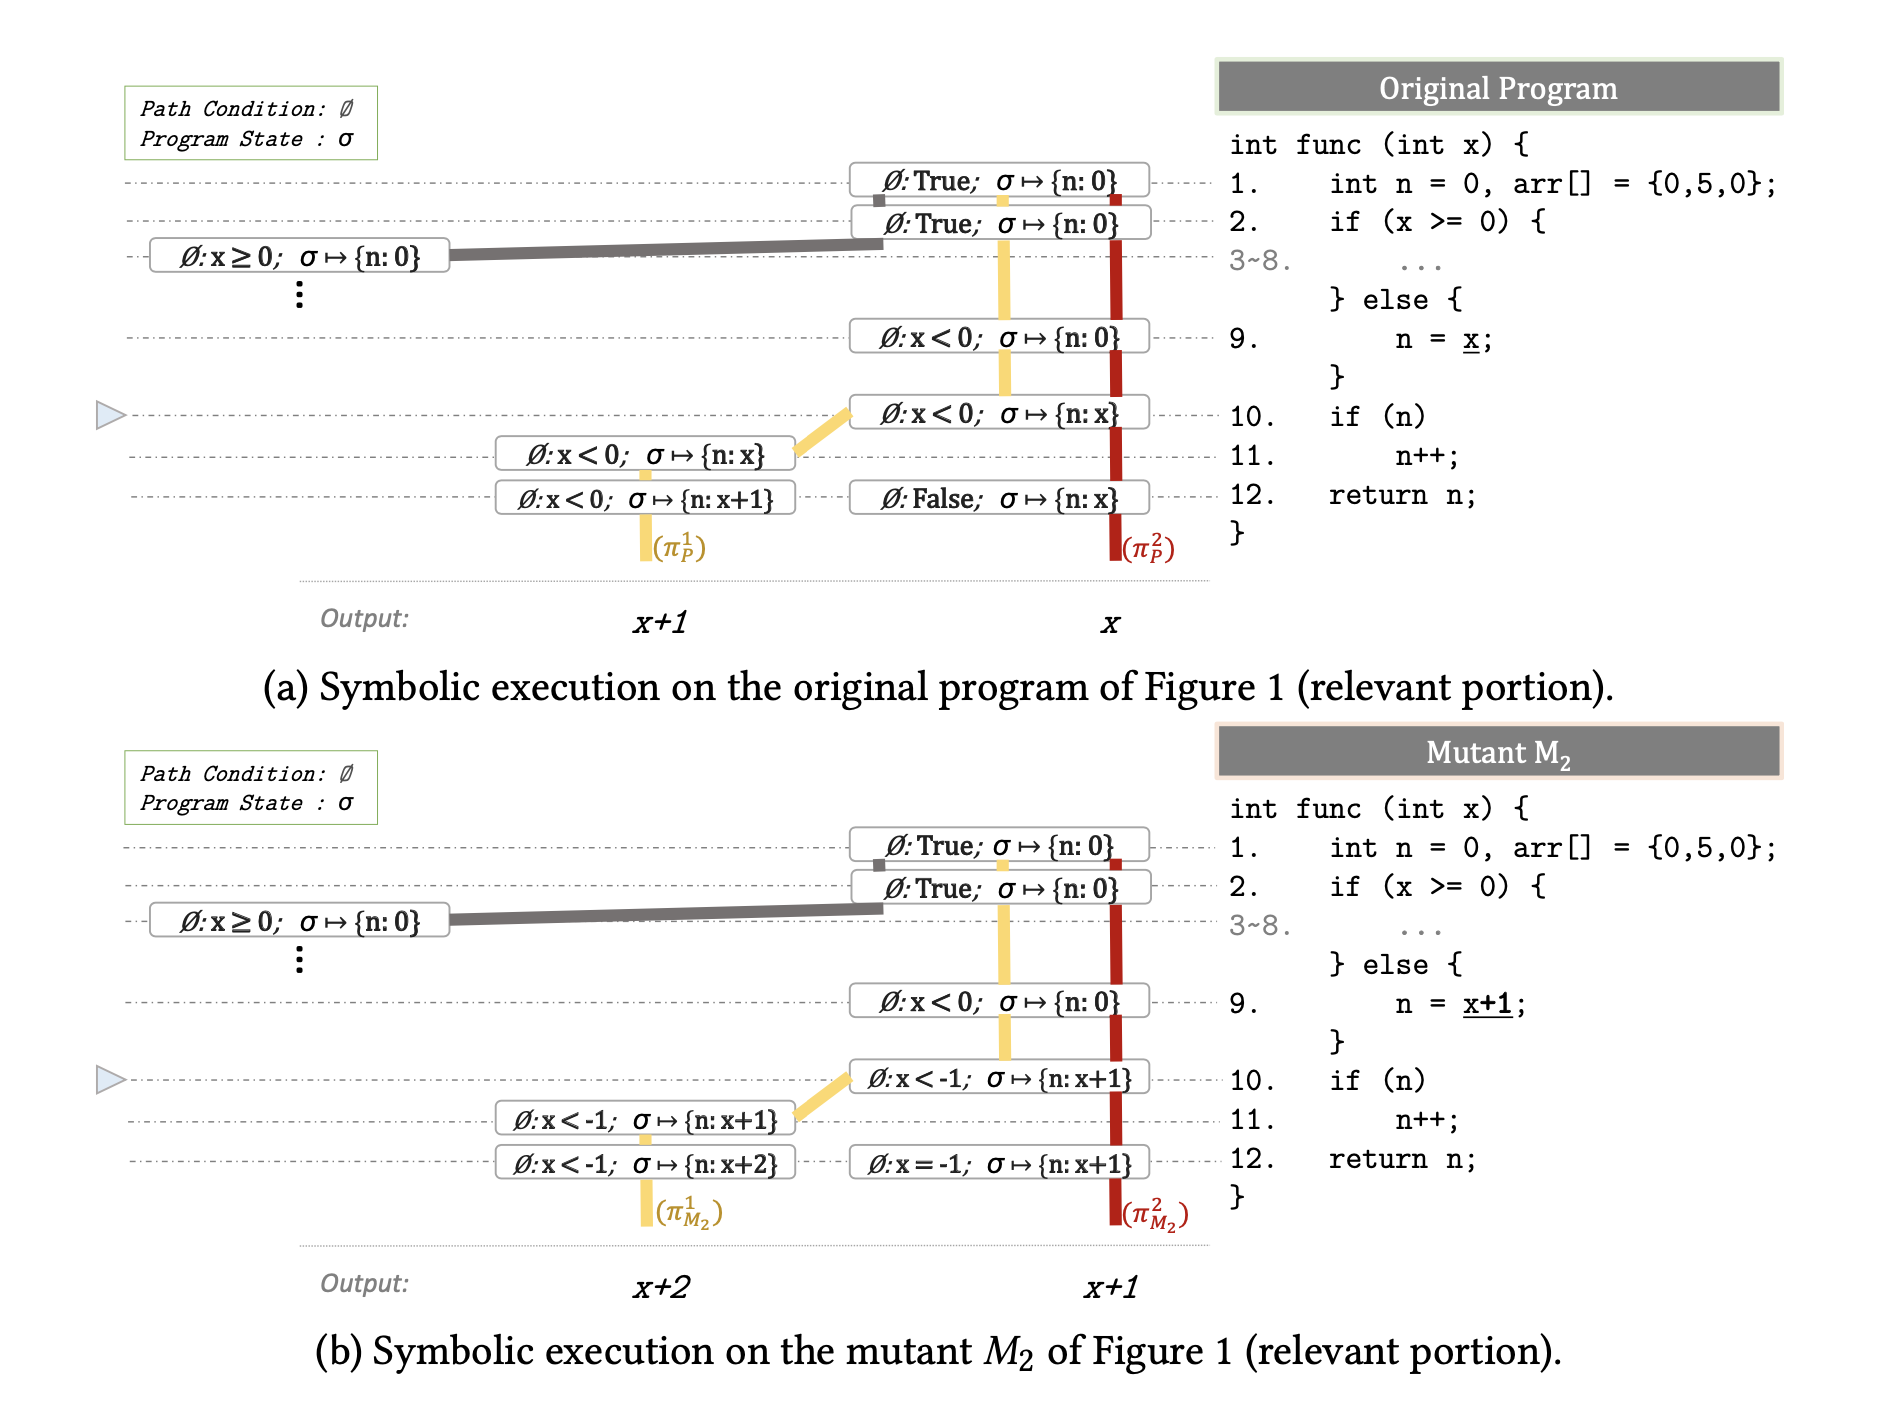
\includegraphics[width=\textwidth]{images/semu-example}
%\caption{SEMu example. Source: Chekam et al.~\cite{chekam2021killing}.}
%\label{fig:semu-example}
%\end{center}
%\end{figure}
%
%Figure~\ref{fig:semu-example} introduces an example of \INDEX{dynamic symbolic execution}, sub-figure (a) shows the symbolic execution for the original program, while (b) shows the symbolic execution process for the mutant version. In order to generate test inputs that kill a mutant, the technique applies symbolic execution to a program $P$ and to its respective mutant $M_2$, to produce their respective symbolic paths. In a second step, the technique solves the formula $kill(\pi_P, \pi_{M_2})$ to generate the test inputs that kills $M_2$ and goes through $\pi_P$ in $P$ and through $\pi_{M_2}$ in $M_2$. 
%As shown in Figure~\ref{fig:semu-example}, symbolic execution on the original program leads to the paths $x < 0$ and $False$, with the respective outputs $x + 1$ and $x$.
%Instead, the symbolic execution on the mutant leads to paths $x < -1$ and $x = -1$, with outputs $x + 2$ and $x + 1$.
%
%Consequently, the only feasible path that targets mutant $M_2$ is the following:
%
%\begin{equation}
%	kill(\pi_{P}^{1}, \pi_{M_2}^{1}) = ((x < 0) \wedge (x + 1 \neq x + 2) )
%\end{equation}
%
%Where the solution to $kill(\pi_{P}^{1}, \pi_{M_2}^{1})$ is $x = -2$.



To speed-up test generation, SEMu integrates a number of optimizations:
\begin{itemize}
	\item \INDEX{Meta-mutation}: all mutants are encoded into a single program called meta-mutant (in FAQAS, we extended it at source code level), the mutant is selected through a branching statement named mutant choice statement.
	\item \textbf{Discarding non-infected mutant paths}: mutant paths failing to infect the program state are discarded immediately.
	\item \textbf{Heuristic search}: stop exploration of a path after $K$ transitions, and solve the kill formula.
	\item \textbf{Infection-only strategy}: Generates test inputs by aiming only at mutant infection.
\end{itemize}

%\DONE{I have the impression that none of the following heuristics are currently used in FAQAS. I would write that we indicate which heuristics are not feasible and which one may be investigated in follow-up activities.}

%To reduce execution time further, SEMu also introduces a list of parametric heuristics that can be controlled by the user; this set of heuristics help to define which paths to explore and in general, the test generation process:

%%\DONE{please use "test cases" not "tests"}
%
%\begin{itemize}
%	\item \textbf{Controlling for reachability} (seeded symbolic execution): This heuristic consists of executing the original program up to a given path using the same inputs provided by existing test cases; the use of concrete inputs helps symbolic execution to quickly prune paths that are infeasible or does not reach the mutant. This feature is inherited from KLEE.
%	%a explore paths in seeded  mode up to a given length. 
%	
%%	\DONE{You are not explained what t does. "This heuristic consists of executing the original program up to a given path using the same inputs provided by existing test cases; it generates symbolic inputs only for...  For its implementation SEMu relies on a feature provided by KLEE"}
%	% This heuristic quickly prunes paths that are infeasible or does not reach the mutant. 
%	
%%	\DONE{Please refine what I wrote in the following. You were not explicitly clrifying hat the problem is.}
%	
%	We do not integrate this feature in the FAQAS framework because of two reasons. 
%	First, SEMu can deal only with test cases for batch programs (i.e., providing arguments to the main function of the software under test), which is different from our context where we either have unit or integration test cases implemented in a specific programming language, or we have complex system test cases simulating communication from ground to orbit through network and a simulator. 
%	Second, in our context, because of the complexity of the SUT we can generate unit test cases but not integration or system level ones. The main difference between such test cases is the entry point, for unit test cases it is the function under test, for integration or system test cases it is a function different than the function under test. Consequently, implementing such solution would require the implementation of additional technology to map the seeds collected for test inputs with different entry points, which is not provided by KLEE.
%
%	\item \textbf{Controlling for propagation}: This heuristic consists of controlling where and how often to verify whether the execution path has propagated the infection (i.e., an erroneous state with respect to the original program) after the execution of the mutated statement; if the mutation does not propagate the infection, the sufficiency killing condition will not be met, and thus it makes sense to prune these paths to decrease the symbolic search space.
%	% sometimes an infected program state fails to propagate the infection to the outputs, these states should be quickly discarded. 
%
%%	\DONE{Rewrite the sentence, unclear}
%	
%	For controlling the propagation of the infected state, SEMu introduces the following four parameters:
%	\begin{itemize}
%%		\item \DONE{(Comments are put above the problematic item) Unclear. Do you want to say that it consider checkpints with a predefined distance? Pleas write complete sentences sbject-verb-object.}
%
%		\item \textbf{Checkpoint Window}: This parameter determines the distance between checkpoints, where checkpoints are program locations with a branching statement. 
%
%		%\DONE{What are the criteria to discard a branch?}
%		At every checkpoint SEMu can (1) discard the branches that failed to propagate the infection, (2) generate tests based on the current states. Not used in FAQAS because we deal with unit testing (i.e., we test the mutated function).
%		
%		%\DONE{There is no more time for investigation, no? Explain why we discard it then.}
%		\item \textbf{Propagating Proportion}: This parameter specifies the percentage of branches that are kept to pursue the exploration. The use of this parameter requires additional investigation, to be investigated in follow-up projects.
%
%
%		%\DONE{You write "these branches", which branches? If all teh heuristics concern finding branches you need to specify above.}
%		%\DONE{To be investigated no}
%		\item \textbf{Propagation Selection Strategy}: While \textbf{Propagating Proportion} specifies the percentage of branches to be selected, this parameter determines how these branches are selected, particularly it can be done (1) randomly, or (2) selecting the branch that is closer to the output. 
%
%		Even though, the random strategy works better with batch programs according to literature~\cite{chekam2021killing}, we deal with unit tests for large programs. 
%
%%		\DONE{Why}
%		\item \textbf{Minimum Propagation Depth (MPD)}: This parameter specifies how many checkpoints should pass before generating the tests. We do not use this parameter in FAQAS (\texttt{MPD = 0}), since this enable SEMu to generate inputs quickly, and thus to save further computation time. 
%	\end{itemize}
%
%%	\DONE{Do not require for dong what? Complete the sentence. Who is the subject?}
%	\item \textbf{Controlling the cost of constraint solving} (no state difference): This heuristic consists of not requiring the state of the original program and the mutant to be different to solve the kill formula. The heuristic is not used in FAQAS, since it lowers the chances of killing a mutant. 
%
%	%\DONE{Unclear. Who is the subject?}
%	\item \textbf{Controlling the number of attempts} (number of tests per mutant): This heuristic specifies the number of tests to be generated for each mutant. Based on the idea that a test can kill multiple mutants. The use of the heuristic in the FAQAS context requires further investigation, to be addressed in follow-up projects. In the meanwhile, we generate only one mutant a time.
%
%\end{itemize}



\subsection{Test Generation based on Evolutionary Computation}

Test generation approaches based on \INDEX{evolutionary computation} typically rely on population-based meta-heuristic optimization algorithms~\cite{harman2011strong}. 
They search for program inputs that could kill mutants under the guidance of a fitness function~\cite{harman2011strong}. 
The main research contribution of these methods is the definition of fitness functions that capture the killing conditions of a mutant and identify test inputs that satisfy those conditions.

The \INDEX{fitness function} captures the killing conditions of a mutant. For instance, Ayari et al.~\cite{ayari2007automatic} proposed to use an evolutionary approach based on \INDEX{ant colony optimization} (ACO) for automatic test input data generation on mutation testing. The ACO is an optimization algorithm inspired by the behavior of ants, it is based on the ants ability to find the shortest path between their nest and the food source. In the study by Ayari et al.~\cite{ayari2007automatic}, the approach takes an existing test case and produces a new test case by slightly modifying its inputs. 
%F: you have to provide more details what does it mean "close"?
The fitness function measures the distance between the mutated statement, and the statement reached by the new test case (e.g., the reachability condition). More precisely, the distance is defined as the number of basic blocks between the two statements in the program's control flow graph.
Papadakis et al.~\cite{papadakis2011automatically}, instead, rely on fitness functions that capture the distance between mutated statement and the statement covering the branches of the different mutations (e.g., the necessity condition).

Fraser and Arcuri~\cite{fraser2015achieving} propose to use distinct distance metrics tailored to the specific operator used to generate the mutants.
%F: we need more examples for multiple operators. Also, you should clarify why distinct metrics are needed
This tailoring is needed because the \EMPH{necessity killing condition} relies on changes in the program state and the execution of a mutated statement does not guarantee that the program state had been changed (i.e., values on the stack are different at the mutation point).
%Fabrizio: it was not comprehensible
%mutation operators change the program state, and in other cases the program state remains unchanged. Because of this, distinct metrics for measuring distance for each operators needs to be defined.
%\DONE{I cannot undertsand the following, we can ignore it.}
%\DONE{In the following, I added a sentence in paranth. Is it correct? YES}
For example, the \textit{deletion operator}, which removes a statement, may or may not change the program state, depending on the semantic of the removed sentence \CHANGEDTWO{(e.g., a logging instruction does not alter the program state)}. In case the mutation effectively changes the program state the distance is set to 0, otherwise the given value is 1.
% For example if the \textit{deletion operator} changes the program state (i.e., values on the stack are different at the mutation point) the distance is 0, otherwise the given value is 1. 
In the case of the \textit{insert unary operator}, which adds or subtracts 1 to a numerical value, the operator always change the program state, so the distance is set to 0 when the statement is reached. 
% For this reason, the mutants produced by this operator always affect the program state, so the distance is always 0 when the statement is reached.

Instead, in the case of the \textit{replace variable operator}, which replaces a specific variable with all other variables of the same type in the program scope, the distance is set to 0 only if the values of the variables being exchanged are different before executing the statement, otherwise it is set to 1.

\subsubsection{\REVTWO{C37}{Generation of test oracles}}
\label{sec:oraclesGeneration:codeDriven}

The automated generation of test oracles is a research topic that goes beyond the specific needs of mutation testing~\cite{Barr:Oracles:15,OLIVEIRA:Oracles:2014}.

Fraser et al. provide an overview of existing approaches for the automated generation of test oracles that have been integrated into existing test case generation tools~\cite{fraser2011mutation}.
A common solution consists of the automated synthesis of assertions for the test case. These assertions reflect the output generated by the function under test when it is exercised with the automatically generated input. 
For example, Line~6 in Listing~\ref{isPositiveOracle} shows the oracle that can be automatically generated for the function analyzed in Listing~\ref{example} (i.e., function \emph{isPositive}). The oracle, in this case, consists of an assertion verifying that the value generated by function \emph{isPositive} matches the value '1', which is the value observed during test generation for the input value '0'. This is the approach implemented by Riener et al.~\cite{riener2011test}, who generate assertions that verify variables that present different values between the original and the mutated executions.

\begin{minipage}{15cm}
\begin{lstlisting}[style=CStyle, caption=Automatically generated oracle for function 'isPositive'., label=isPositiveOracle]
void test () { 
	int numSymbolic = 0;
 	
 	int ret = isPositive(numSymbolic); 
	
	assert( ret == 1 ); 
}
\end{lstlisting}
\end{minipage}

Randoop~\cite{PachecoLEB2007} allows annotation of the source code to identify observer methods to be used for assertion generation. Orstra~\cite{Xie:2006} generates assertions based on observed return values and object states.
DiffGen~\cite{Taneja:2008} extends the Orstra approach to generate assertions from runs on two different program versions.

A well known limitation of automatically generated assertions that reflect the actual values observed during execution is that
they need to be validated. More precisely, we need to ensure that the values expected by the assertions do not reflect a failure triggered by the test case (e.g, an erroneous value being returned). Such validation activity is typically performed manually by the engineers because it should be based on domain knowledge and system specifications. 
Specifications are generally written in natural language because, to reduce development costs, only few components of the system are specified using formal languages. For this reasons the automated verification of such assertions is infeasible.

Approaches that support engineers in the analysis of generated oracles exist and might be considered to speed up the process~\cite{Staats2012,PastoreICSE2015}. For example, 
Staats et al.~\cite{Staats2012} identify the subset of variables to be verified by oracles in order to maximize the fault finding potential of the testing process.
%with respect to the cost of manually verifying the correctness of each generated assertions. 
First, they generate a collection of mutants from the SUT. Second, the test suite (automatically generated) is run against the mutants using the original system as the oracle. Third, they select the variables to verify in test oracles by focussing on those variables that show different values in the original and the mutated version.

ZoomIn.~\cite{PastoreICSE2015} automatically identifies suspicious assertions. These are assertions that verify data that is generated by functions showing anomalies during test cases executions. Anomalies are detected by automatically deriving pre- and post-conditions of the functions of the SUT based on the data recorded during the execution of a manually implemented test suite. Anomalies consist of function executions that violate such pre- and post-conditions. 
%To rank unsafe assertions, ZoomIn takes into consideration the number of violations of pre- and post-conditions produced by the related program variables. However, not all the constraint violations are equally important. Since erroneous behaviors are not frequent in adequately tested software, ZoomIn weights each constraint according to the number of times the constraint has been violated. The frequently violated constraints are likely imprecise constraints that erroneously detect legal values as anomalous values, while constraints that are seldom violated are likely to carry useful information. ZoomIn captures this aspect with the uniqueness score. 
%Also, ZoomIn associates the assertions with a score, the suspiciousness score, that represents the likelihood the assertion is wrong. The suspiciousness score of an assertion depends on both the number and the uniqueness scores of the related constraints that are violated. Intuitively the highly scored assertions, i.e., the most suspicious assertions, are the ones associated with several constraint violations with high uniqueness scores.
%To keep the inspection effort low and the effectiveness high, developers are assumed to inspect only the top assertions in the ranking. Results show that inspecting the top five unsafe assertions is enough to discover several faults without wasting time inspecting too many correct assertions.

% measure how often each variable in the system reveals a fault in a mutant and?based on this information?we rank variable effectiveness in terms of fault finding. Finally, we estimate? based on this ranking?which variables to include in the oracle data for an expected value oracle. The underlying hypothesis is that, as with mutation-based test data selection, oracle data that is likely to reveal faults in the mutants will also be likely to reveal faults in the actual system under test. This oracle data selection process is completely automated and requires no manual intervention. Once this oracle data is selected, the tester defines expected values for each element of the oracle data. Testing then commences with a?hopefully?small and highly effective oracle.


%According to recent survey on the topic, test oracles can be divided in three categories:
%oracles defined though a \INDEX{specification language} (i.e.,  is a notation for defining a specified test oracle, which judges whether the behaviour of a system conforms to a formal specification).

%  test oracles can be derived (Section 5);
%  test oracles can be built from implicit information
%(Section 6); and

%In the context of code-driven metamorphic testing
%
%
%
%Staats2012

\subsection{Summary}

Among all the approaches for test input generation, SEMu is the most advanced one. However, it does not integrate solutions to automatically generate oracles. Solutions for generating oracles are at their infancy and cannot be considered ready for integration into the FAQAS toolset.



